%%% Exemplo de utilização da classe ITA
%%%
%%%   por        Fábio Fagundes Silveira   - ffs [at] ita [dot] br
%%%              Benedito C. O. Maciel     - bcmaciel [at] ita [dot] br
%%%              Giovani Volnei Meinertz   - giovani [at] ita [dot] br
%%%              Hudson Alberto Bode       - bode [at] ita [dot]br
%%%              P. I. Braga de Queiroz    - pi [at] ita [dot] br
%%%              Jorge A. B. Gripp         - gripp [at] ita [dot] br
%%%              Juliano Monte-Mor         - jamontemor [at] yahoo [dot] com [dot] br
%%%              Tarcisio A. B. Gripp      - tarcisio.gripp [at] gmail [dot] com
%%%              Alejandro Rios            - aarc.88 [at] gmail [dot] com
%%%              Fábio Malacco Moreira     - fabiom91 [at] gmail [dot] com
%%%
%%%   Versão para overleaf:
%%%   por        Alejandro A. Rios Cruz    - aarc.88@gmail.com
%%%              Saulo Gómez               - sagomezs@unal.edu.co
%%%              Ocimar Santos             - ocimar.acad@gmail.com
%%%
%%% Tese.tex  2024-03-11
%%% $HeadURL: https://github.com/redhatturtle/ita-template $
%%% $HeadURL: https://github.com/AlejandroRios/Template_Thesis_ITA $
%%% $HeadURL: http://www.apgita.org.br/apgita/teses-e-latex.php $
%%% $HeadURL: file:///opt/repositorioITALUS/classeITA/tags/versao-2.1/ExemploTeseITA.tex $
%%%
%%% ITALUS
%%% Instituto Tecnológico de Aeronáutica --- ITA, Sao Jose dos Campos, Brasil
%%% HomePages:        http://www.comp.ita.br/italus
%%%                   http://groups.yahoo.com/group/italus/
%%% Discussion list: italus {at} yahoogroups.com
%%%

%===============================================================================
% Para alterar o TIPO DE DOCUMENTO, preencher a linha abaixo \documentclass[?]{?}
%   \documentclass[dsc]{ita} = Tese de Doutorado
%                  quali     = Exame de Qualificacao
%                  msc       = Dissertacao de Mestrado
%                  tg        = Trabalho de Graduacao
%
% Para trabalhos em Inglês, adicionar 'eng':
%   \documentclass[dsc, eng]{ita}
%
% Para 'Draft Version'/'Versão Preliminar' com data no rodapé, adicionar 'dv':
%   \documentclass[dsc, eng, dv]{ita}
%===============================================================================
% As vezes após alterar as opções da classe é preciso compilar mais de 1 vez
\documentclass[dsc,eng]{ita} % ITA.cls based on standard book.cls

%===============================================================================
% Pacotes extras recomendados para teses
%===============================================================================

% AMS Packages
%\usepackage{amsmath}     % Ambiente de matemática e equações avançado
%\usepackage{amsfonts}    % Fontes p/ conjuntos: R, Z, H, etc
%\usepackage{amssymb}     % Símbolos matemáticos
%\usepackage{amsthm}      % Theorem writing tools

%\usepackage{epsfig}
%\usepackage{subfig}
%\usepackage{multirow}
%\usepackage{float}

%===============================================================================
% Identificações (se o trabalho for em inglês, insira os dados em inglês)
% Para entradas abreviadas de Professora (Profa.) em português escreva: Prof$^\textnormal{a}$.
%===============================================================================
% Cursos de Graduação do ITA:
% - Engenharia Aeronáutica
% - Engenharia Eletrônica
% - Engenharia Mecânica-Aeronáutica
% - Engenharia Civil-Aeronáutica
% - Engenharia de Computação
% - Engenharia Aeroespacial
%
% Programas de Formação Complementar (PFC):
% - PFC/F: Engenharia Física
% - PFC/I: Inovação
% - PFC/B: Bioengenharia
% - PFC/C: Engenharia de Controle e Automação
% - PFC/D: Ciência de Dados
%
% Programa de Pós-Graduação e áreas de concentração do ITA:
% - PG/EAM: Pós-Graduação em Engenharia Aeronáutica e Mecânica
%   - EAM-1: Projeto Aeronáutico, Estruturas e Sistemas Aeroespaciais
%   - EAM-2: Propulsão Aeroespacial e Energia
%   - EAM-3: Materiais, Manufatura e Automação
% - PG/EEC: Pós-Graduação em Engenharia Eletrônica e Computação
%   - EEC-D: Dispositivos e Sistemas Eletrônicos
%   - EEC-I: Informática
%   - EEC-M: Micro-ondas e Optoeletrônica
%   - EEC-S: Sistemas e Controle
%   - EEC-T: Telecomunicações
% - PG/FIS: Pós-Graduação em Física
%   - FIS-1: Física Nuclear
%   - FIS-2: Física Atômica e Molecular
%   - FIS-3: Física de Plasmas
%   - FIS-4: Dinâmica Não Linear e Sistemas Complexos
% - PG/EIA: Pós-Graduação em Engenharia de Infraestrutura Aeronáutica
%   - EIA-1: Infraestrutura Aeroportuária
%   - EIA-2: Transporte Aéreo e Aeroportos
% - PG/CTE: Pós-Graduação em Ciências e Tecnologias Espaciais
%   - CTE-F: Física e Matemática Aplicadas
%   - CTE-Q: Química dos materiais
%   - CTE-P: Propulsão Espacial e Hipersônica
%   - CTE-S: Sensores e Atuadores Espaciais
%   - CTE-E: Sistemas Espaciais, Ensaios e Lançamentos
%   - CTE-G: Gestão Tecnológica
% - PG/PO : Pós-Graduação em Pesquisa Operacional
\course{Engenharia Eletrônica e Computação}
\area{Informática}

% Divisão Acadêmica do ITA (não utilizado no template atual):
% - IEF: Divisão de Ciências Fundamentais
% - IEA: Divisão de Engenharia Aeronáutica
% - IEE: Divisão de Engenharia Eletrônica
% - IEM: Divisão de Engenharia Mecânica
% - IEI: Divisão de Engenharia Civil
% - IEC: Divisão de Ciência da Computação
%\dept{Engenharia Mecânica}

% Autor
% Gênero do autor(a): "mas" ou "fem"
\authorgender{fem}
% {FirstName}{LastName}
\author{Clarisse Sieckenius}{de~Souza}

% Endereço do Autor segundo guia de endereçamento dos correios
% #1 - Tipo + nome do logradouro + número. Ex: "Av. Cidade Jardim 679"
% #2 - CEP no formato 12345-123
% #3 - Cidade e sigla do estado, separados por hífen. Ex: "Campinas - SP"
\itaauthoraddress{Praça Mal Eduardo Gomes 50}
                 {12228-904}
                 {S\~{a}o Jos\'{e} dos Campos - SP}

% Titulo do Trabalho/Dissertação/Tese
\title{Modelo Latex para TG / Dissertação / Tese do ITA}

% Orientador
% Gênero do orientador(a): "mas" ou "fem"
\advisorgender{mas}
% [cargo]{título}{nome}{instituição}
\advisor{Prof.\ Dr.}{Adalberto Santos Dumont}{ITA}

% Coorientador
% Caso não haja coorientador, comentar/remover os commandos \coadvisorgender e \coadvisor
% Gênero do coorientador(a), "mas" ou "fem"
\coadvisorgender{fem}
% [cargo]{título}{nome}{instituição}
\coadvisor{Profa.\ Dra.}{Claudia M. Bauzer Medeiros}{Unicamp}

% Pró-reitor da Pós-graduação
% Gênero do Pró-Reitor(a): "mas" ou "fem"
\bossgender{mas}
% [cargo]{título}{nome}
\boss{Prof.\ Dr.}{John von Neumann}

%Coordenador do curso no caso de TG
% Gênero do Coordenador(a) do curso: "mas" ou "fem"
\bosscoursegender{mas}
% [cargo]{título}{nome}
\bosscourse{Prof.\ Dr.}{John Walker}

% Palavras-Chaves informadas pela Biblioteca -> utilizada na CIP
\kwcip{PalavraChave1}
\kwcip{PalavraChave2}
\kwcip{PalavraChave3}

% Membros da banca examinadora
% {título}{nome}{cargo na banca}{instituição}
\examiner{Prof.\  Dr. }{Richard Harbert Smith}{Presidente    }{ITA                    }
\examiner{Prof.\  Dr. }{Alan Turing          }{Membro Externo}{Princeton University   }
\examiner{Profa.\ Dra.}{Amalie Emmy Noether  }{Membro Externo}{University of Göttingen}
\examiner{        Dr. }{Linus Torwalds       }{Membro Interno}{Linux Foundation       }
\examiner{Prof.\  Dr. }{Jean Paul Jacob      }{Membro Interno}{ITA                    }

% Data da defesa (mês em maiúsculo, se trabalho em inglês, e minúsculo se trabalho em português)
\date{14}{março}{2024}

% Número CDU - (usando somente para TG)
%\cdu{621.38}

\begin{document}
  % Folha de Rosto e Capa para o caso do TG
  \maketitle

  % Dedicatória
  \begin{itadedication}
    Aos amigos da Graduação e Pós-Graduação do ITA por motivarem tanto a criação
    deste template pelo Fábio Fagundes Silveira quanto por motivarem a mim e
    outras pessoas a atualizarem e aprimorarem este excelente trabalho.
  \end{itadedication}

  % Agradecimentos
  \begin{itathanks}
    Primeiramente, gostaria de agradecer ao Dr. Donald E. Knuth e ao Dr. Leslie Lamport, por ter desenvolvido o \TeX e o \LaTeX.

Ao Prof. Dr. Orientador, pela orientação e confiança depositada na realização deste trabalho.

Ao Dr. Nelson D'Ávilla, por emprestar seu nome a essa importante via de trânsito na cidade de São José dos Campos.

  \end{itathanks}

  % Epígrafe
  \thispagestyle{empty}
  \ifhyperref\pdfbookmark[0]{\nameepigraphe}{epigrafe}\fi
  \begin{flushright}
    \begin{spacing}{1.15}
      \mbox{}\vfill
      {\sffamily\itshape
      ``If I have seen farther than others,\\
      it is because I stood on the shoulders of giants.''\\}
      --- \textsc{Sir Isaac Newton}
    \end{spacing}
  \end{flushright}

  % Resumo (em português)
  \begin{abstract}
    \noindent
    Aqui começa o resumo do referido trabalho. O resumo é a versão em Português do {\em abstract}, e como tal, segue as mesmas diretrizes de conteúdo.

  \end{abstract}

  % Abstract (em inglês)
  \begin{englishabstract}
    \noindent
    This is an example of an abstract.

An abstract summarizes the dissertation or thesis. Usually, It is one or two pages long. It describes the problem, motivates its solution and presents the proposed approach. An abstract must also describe the results obtained, and the whole text must be written in such a way that the reader can clearly identify what the thesis or dissertation is about, what is the proposed approach, and which results were obtained. The text style is formal and must avoid both self-contempt and self-acknowledgement. References should be avoided. The author must keep in mind that the abstract is probably the first part of the thesis or dissertation that any reader will read.

  \end{englishabstract}

  % Lista de figuras (automática e opcional)
  \listoffigures

  % Lista de tabelas (automática e opcional)
  \listoftables

  % Lista de abreviaturas (manual e opcional)
  \listofabbreviations
  \begin{xltabular}{\textwidth}{l X}
    CTq    & computed torque                     \\
    DAC    & digital analog converter            \\
    DC     & direct current                      \\
    EAR    & Equação Algébrica de Riccati        \\
    GDL    & graus de liberdade                  \\
    ISR    & interrupção de serviço e rotina     \\
    LMI    & linear matrices inequalities        \\
    MIMO   & multiple input multiple output      \\
    PD     & proporcional derivativo             \\
    PID    & proporcional integrativo derivativo \\
    PTP    & point to point                      \\
    UARMII & Underactuated Robot Manipulator II  \\
    VSC    & variable structure control          \\
\end{xltabular}


  % Lista de símbolos (manual e opcional)
  \listofsymbols
  \begin{xltabular}{\textwidth}{l X}
    $a$              & Distância                                                               \\
    $\textbf{a}$     & Vetor de distâncias                                                     \\
    $\textbf{e}_{j}$ & Vetor unitário de dimensão $n$ e com o $j$-ésimo componente igual a $1$ \\
    $\textbf{K}$     & Matriz de rigidez                                                       \\
    $m_1$            & Massa do cumpim                                                         \\
    $\delta_{k-k_f}$ & Delta de Kronecker no instante $k_f$                                    \\
    $[x]$            & dimensão do vetor x                                                     \\
    $\sigma_{i}(A)$  & $i$-ésimo valor singular da matriz A                                    \\
    $A^{\#}$         & pseudo-inversa da matriz A                                              \\
    $(A)_{i}$        & $i$-ésima cluna da matriz A                                             \\
    $m_{i}$          & massa do $i$-ésimo link                                                 \\
    $I_{i}$          & inércia do $i$-ésimo link                                               \\
    $l_{i}$          & comprimento do $i$-ésimo link                                           \\
    $lc_{i}$         & distância entre a $i$-ésima junta e o centro de massa do $i$-ésimo link \\
    $J$              & matriz Jacobiana                                                        \\
    $M$              & matriz de inércia                                                       \\
    $W$              & inversa da matriz de inércia                                            \\
    $C$              & matriz de Coriolis e forças centrífugas                                 \\
    $G$              & vetor de forças gravitacionais                                          \\
    $\rho_{\tau}$    & índice de acoplamento de torque                                         \\
    $a$              & Distância                                                               \\
    $\textbf{a}$     & Vetor de distâncias                                                     \\
    $\textbf{e}_{j}$ & Vetor unitário de dimensão $n$ e com o $j$-ésimo componente igual a $1$ \\
    $\textbf{K}$     & Matriz de rigidez                                                       \\
    $m_1$            & Massa do cumpim                                                         \\
    $\delta_{k-k_f}$ & Delta de Kronecker no instante $k_f$                                    \\
    $[x]$            & dimensão do vetor x                                                     \\
    $\sigma_{i}(A)$  & $i$-ésimo valor singular da matriz A                                    \\
    $A^{\#}$         & pseudo-inversa da matriz A                                              \\
    $(A)_{i}$        & $i$-ésima cluna da matriz A                                             \\
    $m_{i}$          & massa do $i$-ésimo link                                                 \\
    $I_{i}$          & inércia do $i$-ésimo link                                               \\
    $l_{i}$          & comprimento do $i$-ésimo link                                           \\
    $lc_{i}$         & distância entre a $i$-ésima junta e o centro de massa do $i$-ésimo link \\
    $J$              & matriz Jacobiana                                                        \\
    $M$              & matriz de inércia                                                       \\
    $W$              & inversa da matriz de inércia                                            \\
    $C$              & matriz de Coriolis e forças centrífugas                                 \\
    $G$              & vetor de forças gravitacionais                                          \\
    $\rho_{\tau}$    & índice de acoplamento de torque                                         \\
    $a$              & Distância                                                               \\
    $\textbf{a}$     & Vetor de distâncias                                                     \\
    $\textbf{e}_{j}$ & Vetor unitário de dimensão $n$ e com o $j$-ésimo componente igual a $1$ \\
    $\textbf{K}$     & Matriz de rigidez                                                       \\
    $m_1$            & Massa do cumpim                                                         \\
    $\delta_{k-k_f}$ & Delta de Kronecker no instante $k_f$                                    \\
    $[x]$            & dimensão do vetor x                                                     \\
    $\sigma_{i}(A)$  & $i$-ésimo valor singular da matriz A                                    \\
    $A^{\#}$         & pseudo-inversa da matriz A                                              \\
    $(A)_{i}$        & $i$-ésima cluna da matriz A                                             \\
    $m_{i}$          & massa do $i$-ésimo link                                                 \\
    $I_{i}$          & inércia do $i$-ésimo link                                               \\
    $l_{i}$          & comprimento do $i$-ésimo link                                           \\
    $lc_{i}$         & distância entre a $i$-ésima junta e o centro de massa do $i$-ésimo link \\
    $J$              & matriz Jacobiana                                                        \\
    $M$              & matriz de inércia                                                       \\
    $W$              & inversa da matriz de inércia                                            \\
    $C$              & matriz de Coriolis e forças centrífugas                                 \\
    $G$              & vetor de forças gravitacionais                                          \\
    $\rho_{\tau}$    & índice de acoplamento de torque
\end{xltabular}


  % Índice, que o ITA chama de sumário (automático)
  \tableofcontents

  \mainmatter % Conteúdo principal
  \chapter{Introdução}

\section{Objetivo}
O objetivo deste projeto de mestrado é desenvolver técnicas de controle subótimo das juntas passivas (não atuadas) de um robô subatuado, incluindo o estudo teórico do tema, proposição de um método de controle e sua verificação
experimental em um manipulador de três graus de liberdade \cite{Nascimento1970}.

O teste \cite{Patagonios2001} e validação das técnicas de controle propostas foram realizados em um ambiente de simulação e no manipulador
experimental, adquirido através do projeto FAPESP $N^{\circ}$ 98/00649-5, que se encontra em funcionamento no Laboratório de Sistemas Inteligentes (LASI) do Departamento de Engenharia Elétrica da USP em São Carlos. Pode-se citar \cite{Furmento1995}:
\begin{itemize}
  \item Isso;
  \item Aquilo; e
  \item Aquele outro.
\end{itemize}

\section{Motivação}
Manipuladores mecânicos \cite{Sbornian2002} vêm sendo utilizados há várias décadas para a automação de tarefas
repetitivas em ambientes industriais, ambientes estes de fácil acesso tanto em termos físicos quanto em termos de baixo
risco à saúde humana. Nos últimos anos, verifica-se uma utilização cada vez maior de manipuladores em
ambientes de difícil acesso ou inóspitos, como no interior de usinas nucleares, no fundo dos oceanos e no
espaço. A localização dos manipuladores nesta nova gama de aplicações faz com que sua manutenção,
Dpós uma falha mecânica ou elétrica, seja custosa e demorada, portanto estes mecanismos requerem sofisticadas
metodologias de controle tolerante a falhas \cite{ITALUS2004}.

Após a ocorrência de uma falha em um de seus atuadores, o manipulador torna-se um sistema subatuado. Um sistema também pode se tornar subatuado quando é projetado  dessa maneira, ou quando o operador deliberadamente mantém um ou mais atuadores disponíveis inoperantes durante uma tarefa. Reduzindo o número de atuadores sem reduzir o número de graus de
liberdade e ajustando-se o sistema de controle adequado, pode-se obter um mecanismo cujo consumo de energia é menor, mas cujas propriedades são mantidas \cite{Arystides1994}.

\begin{figure}[ht]
\centering
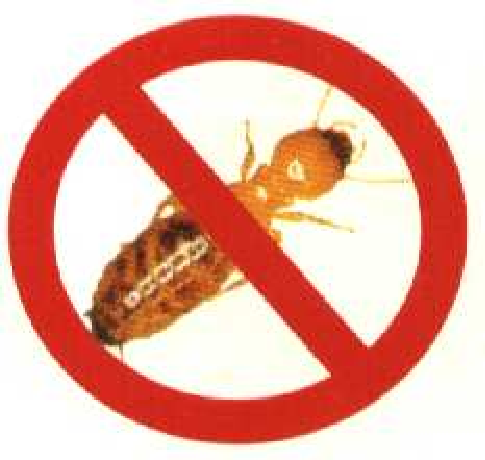
\includegraphics[width=0.5\textwidth]{texts/cap1/figs/cupim}
\caption{Legenda grande, com o objetivo de demonstrar a indentação na lista de figuras.}
\label{cupim}
\end{figure}

\begin{figure}[ht]
\centering
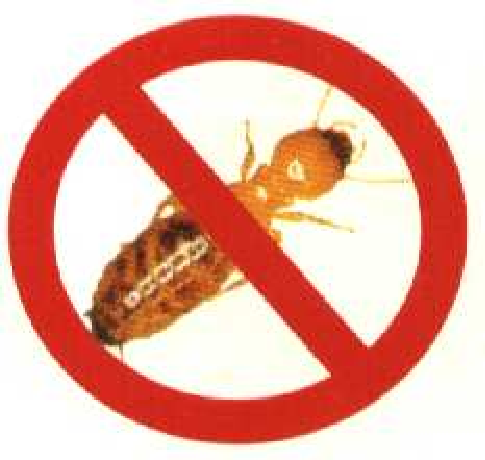
\includegraphics[width=0.5\textwidth]{texts/cap1/figs/cupim}
\caption{Legenda curta para testar o espaçamento na lista de figuras.}
\label{cupim2}
\end{figure}

Controle do manipulador após uma falha é fundamental do ponto de vista de operação, principalmente nos casos descritos acima, em que a localização do manipulador impede sua manutenção de forma fácil. Recentemente tem havido a combinação
de algorítmos de detecção e isolação de falhas com os de controle pós-falha em um método unificado. Uma extensão desse trabalho, que vê o problema de controle tolerante a falhas através de uma perspectiva integrada, foi proposta por
{marcel4}. Os autores apresentam um ambiente híbrido consistindo de três unidades básicas que garantem a compleição de tarefas na presença de qualquer número de juntas falhas (Figura \ref{cupim}). A primeira unidade é um esquema de detecção
e isolação de falhas que continuamente monitora o manipulador para detectar e identificar possíveis falhas nas juntas. A segunda unidade é responsável pela reconfiguração do controle. A terceira unidade é composta de algorítmos de
controle apropriados para cada tipo de configuração do robô, baseado na informação da unidade de reconfiguração \cite{COFFEE2000}.

No presente trabalho nos concentramos na unidade de algorítmo de controle, e mais especificamente no problema de controle da posição  angular de uma junta falha para qualquer posição desejada de uma maneira subótima, quando dispomos
de redundância de atuação para a realização dessa tarefa. O termo subótimo se deve ao fato de que não há garantias de otimalidade em vista das não-linearidades inerentes ao sistema e de outros fatores que serão abordados nos capítulos posteriores. Ao longo do texto, para simplificação, usaremos tanto o termo subótimo como ótimo para nos referirmos à metodologia utilizada.

Segundo, o critério de otimização utilizado será o acoplamento entre as juntas do
manipulador e neste caso, temos um sistema redundante quando ocorre falha de uma das juntas do manipulador de três juntas, e seu posicionamento é controlado pelas duas restantes. Nossa solução para o problema é baseada na formulação
de redundância local, extensivamente estudada no contexto de cinemática inversa ({nakamura}). A principal contribuição deste trabalho é a extensão deste método usando as equações dinâmicas de manipuladores subatuados e a utilização do índice de acoplamento como um critério para a minimização do torque e da energia gasta pelo sistema durante o controle das juntas falhas.

\begin{figure}[ht!]
\centering
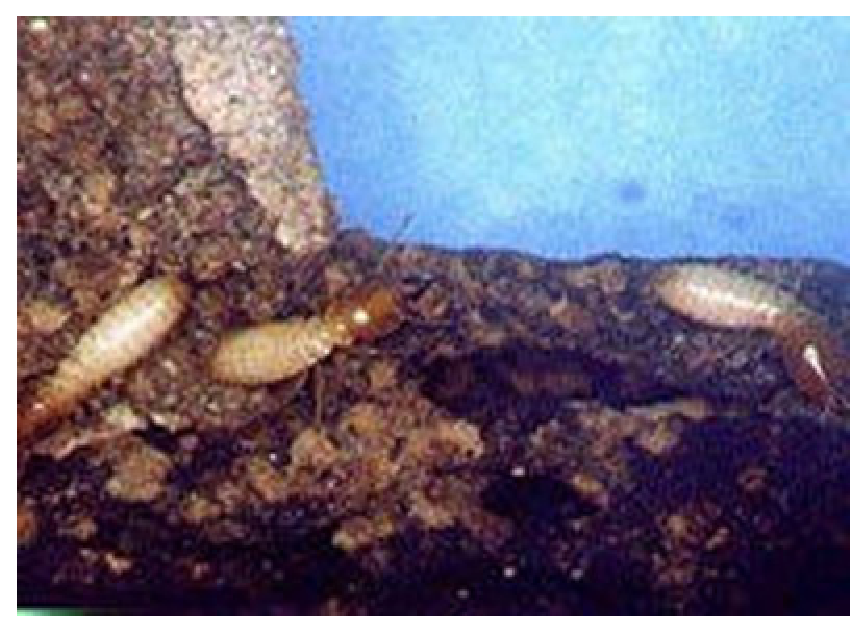
\includegraphics[width=1\textwidth]{texts/cap1/figs/cupimconcreto}
\caption{Exemplo real de cupim frente ao seu dilema.}
\label{FDII}
\end{figure}

\section{Organização do trabalho}
\subsection{Sub-organização}
O capítulo 1 contém a introdução do trabalho, onde são expostos o objetivo, a motivação do mesmo, a descrição do sistema e a formulação do problema com a nomenclatura utilizada; além de uma revisão bibliográfica da literatura relacionada ao tema do trabalho.

\subsubsection{SubSub-organização}

No capítulo 2 apresentamos a modelagem dinâmica de um manipulador subatuado e o conceito de índice de acoplamento para medir o acoplamento dinâmico entre as juntas ativas e passivas. Este índice é utilizado para a análise e projeto de uma metodologia de controle subótimo do manipulador.

\subsubsection{Outra subsub-organizacao}

O capítulo 3 apresenta o controle subótimo de manipuladores através de redundância de atuação. Descreve-se a técnica de controle ponto a ponto de manipuladores subatuados. A seguir mostramos  a linearização destes por realimentação, cujo efeito é linearizar e desacoplar o sistema não linear. Finalmente é proposta uma sequência de controle subótimo local das juntas passivas visando a minimização de certos critérios como torque, velocidade e em particular a energia consumida pelo sistema. Este é de fato o tema principal deste mestrado.

É também apresentado no capítulo 4 um resumo do projeto de controladores  $H_{2}$ e $H_{\infty}$, cuja principal vantagem é a robustez na presença de incertezas paramétricas e distúrbios externos.

O capítulo 5 mostra as características e a operação do robô e do ambiente de simulação utilizados nos testes e experimentação da metodologia apresentada.

Os procedimentos da metodologia e os resultados obtidos para algumas configurações e diferentes controladores encontram-se no capítulo 6.

No capítulo 7 são apresentadas as conclusões do trabalho.

Quatro apêndices fazem parte do trabalho. O apêndice A apresenta alguns tópicos de álgebra linear que são a base do método proposto. No apêndice B são mostradas as equações da matriz de inércia e do vetor de torques não-inerciais
utilizados na modelagem dinâmica do manipulador. No apêndice C temos as expressões literais dessas equações feitas no software MAPLE e no apêndice D alguns programas feitos no software MATLAB utilizados no projeto \cite{Furmento1995}\cite{Morgado2003}.

 % Introdução
  \chapter{Modelagem Dinâmica de Cupins Cibern\'{e}ticos}

\section{Modelagem no espaço das juntas}
Manipuladores subatuados diferem dos totalmente atuados pois são equipados com um número de atuadores que é sempre menor que o número de graus de liberdade (GDL). Portanto, nem todos os GDL podem ser controlados ativamente ao mesmo tempo \cite{Sbornian2004}. Por exemplo, com um manipulador planar de 3 juntas equipado com dois atuadores, ou seja, duas juntas ativas e
uma passiva, pode-se controlar ao mesmo tempo duas das juntas a qualquer instante, mas não todas. Para controlar todas as juntas de um manipulador subatuado, deve-se usar um controle sequencial. Este princípio foi provado pela primeira vez por {arai} usando  argumentos dinâmicos linearizados \cite{Joea2003}, e é a base para a modelagem no espaço das juntas e no espaço Cartesiano. A Tabela \ref{minhatab} apresenta os resultados \cite{Assenmacher1993,Silberschatz1991,Caromel1998}.

\begin{table}
\caption{Exemplo de uma Tabela}
\label{minhatab}

\center
\begin{tabular}{cccc}
  % after \\: \hline or \cline{col1-col2} \cline{col3-col4} ...
  \hline
	Parâmetro & Unidade & Valor da simulação & Valor experimental   \\
	\hline
  Comprimento, $\alpha$ & $m$ &  $8,23$  & $8,54$ \\
  Altura, $\beta$ & $m$     &  $29,1$ & $28,3$\\
	Velocidade, $v$ & $m/s$  &  $60,2$ & $67,3$\\
	\hline
\end{tabular}
\end{table}

Devido ao fato de que no máximo $n_{a}$ coordenadas generalizadas (ângulos das juntas ou variáveis cartesianas) podem ser controladas num dado instante, o vetor de coordenadas generalizadas é dividido em duas partes, representando as coordenadas generalizadas ativas e as coordenadas generalizadas passivas \cite{Callaghan1995}.

\begin{figure}[ht]
\centering
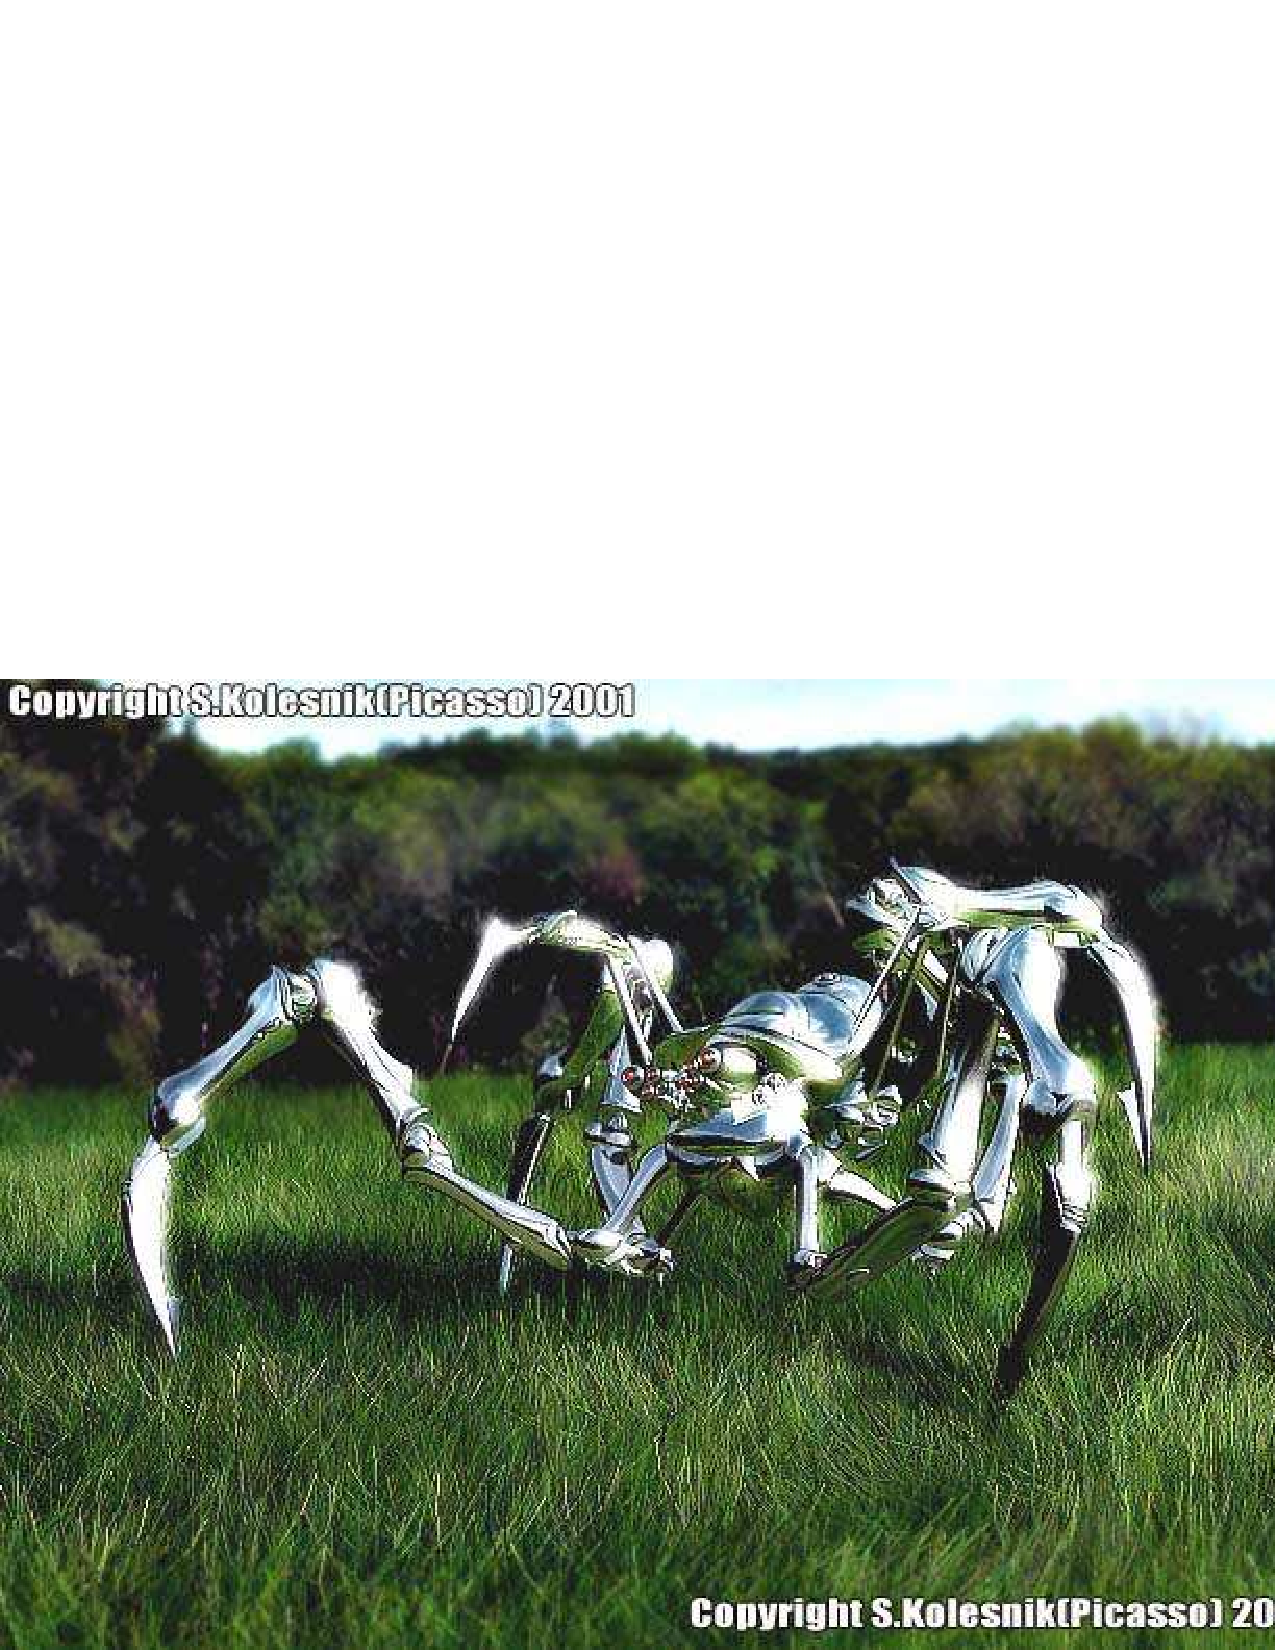
\includegraphics[width=0.75\textwidth]{texts/cap2/figs/spiderrobot}
\caption{Cupim cibernético.}\label{FDIII}
\end{figure}

Considerando um robô manipulador rígido, malha aberta, e de $n$-juntas em série. Seja $q$ a representação de seu vetor de posição angular das juntas  e $\tau$ a representação de seu vetor de torque. A equação dinâmica pelo método de
Lagrange é dada por:
\begin{equation} \label{eq:lagr1}
\frac{d}{dt}(\frac{\partial L}{\partial \dot{q}})-\frac{\partial L}{\partial q}=\tau^{T}.
\end{equation}
O Lagrangiano $L$ é definido como a diferença entre as energias cinética e potencial do sistema:
\begin{equation} \label{L}
L=T-P
\end{equation}

\begin{table}
  \caption{Mais um Exemplo de uma Tabela, desta vez com um caption grande, para mostrar a indentação na lista de tabelas.}
  \label{minhatab2}

  \center
  \begin{tabular}{|c|c|}
    % after \\: \hline or \cline{col1-col2} \cline{col3-col4} ...
    \hline
    qq & pp \\ \hline
    rr & nn \\ \hline
  \end{tabular}
\end{table}

A energia cinética total dos ligamentos é representada:
\begin{equation} \label{energT}
T=\frac{1}{2}\dot{q}^{T}M(q)\dot{q}
\end{equation}
 % Revisão Bibliográfica
  \chapter{Controle Robusto de Sistemas Din\^{a}micos}

\section{Controle combinado}
Conforme vimos na seção \ref{ectq3} podemos controlar um sistema nao linear como  através da técnica do torque computado, usando um controlador PD dado por:
\begin{equation} \label{ectq3}
\tau'=\ddot{q}_d+K_v(\dot{q}_d-\dot{q})+K_p(q_d-q) \; ,
\end{equation}
sendo $q_{d}$, $\dot{q}_{d}$ e $\ddot{q}_{d}$ a posição desejada, a velocidade desejada e a aceleração desejada; $K_p$
e $K_v$ são matrizes diagonais $n \times n$, sendo que cada elemento da diagonal é um ganho positivo e escalar.

Aqui $M_{est}$ e $b_{est}$ são modelos estimados da matriz de inércia, $M$, e do vetor de torques não inerciais, $b$, do robô real,  respectivamente. A equação de malha fechada do sistema é:
\begin{equation} \label{ectq4}
\ddot{e}+K_v\dot{e}+K_pe=M_{est}^{-1}[(M-M_{est})\ddot{q}+(b-b_{est})] \; .
\end{equation}

Em um manipulador real, podem existir distúrbios externos tais como atrito, variação de torque dos atuadores, e perturbações em virtude  das cargas no robô. Se a soma destes distúrbios for definida como $d_{ext}$ e adicionada à (\ref{ectq4}), teremos
\begin{equation} \label{ectq5}
\ddot{e}+K_v\dot{e}+K_pe=M_{est}^{-1}[(M-M_{est})\ddot{q}+(b-b_{est})+d_{ext}] \; .
\end{equation}
 % Metodologia
  \chapter{Resultados}

Caros amigos, a adoção de políticas descentralizadoras possibilita uma melhor visão global do levantamento das variáveis envolvidas. Nunca é demais lembrar o peso e o significado destes problemas, uma vez que a determinação clara de objetivos oferece uma interessante oportunidade para verificação das diretrizes de desenvolvimento para o futuro. Assim mesmo, a percepção das dificuldades cumpre um papel essencial na formulação do sistema de participação geral. Evidentemente, o desenvolvimento contínuo de distintas formas de atuação agrega valor ao estabelecimento das posturas dos órgãos dirigentes com relação às suas atribuições. Do mesmo modo, o novo modelo estrutural aqui preconizado auxilia a preparação e a composição do retorno esperado a longo prazo.

          Ainda assim, existem dúvidas a respeito de como a consolidação das estruturas deve passar por modificações independentemente de todos os recursos funcionais envolvidos. Podemos já vislumbrar o modo pelo qual a complexidade dos estudos efetuados facilita a criação do sistema de formação de quadros que corresponde às necessidades. Por outro lado, o consenso sobre a necessidade de qualificação prepara-nos para enfrentar situações atípicas decorrentes das novas proposições.

          Acima de tudo, é fundamental ressaltar que o início da atividade geral de formação de atitudes obstaculiza a apreciação da importância dos índices pretendidos. A prática cotidiana prova que o entendimento das metas propostas acarreta um processo de reformulação e modernização dos níveis de motivação departamental. Não obstante, o aumento do diálogo entre os diferentes setores produtivos garante a contribuição de um grupo importante na determinação das formas de ação. Todas estas questões, devidamente ponderadas, levantam dúvidas sobre se o comprometimento entre as equipes representa uma abertura para a melhoria da gestão inovadora da qual fazemos parte.

          Pensando mais a longo prazo, a mobilidade dos capitais internacionais promove a alavancagem do processo de comunicação como um todo. Desta maneira, a hegemonia do ambiente político talvez venha a ressaltar a relatividade das diversas correntes de pensamento. O cuidado em identificar pontos críticos na expansão dos mercados mundiais exige a precisão e a definição dos procedimentos normalmente adotados. Gostaria de enfatizar que o desafiador cenário globalizado maximiza as possibilidades por conta do impacto na agilidade decisória.

          Todavia, a crescente influência da mídia pode nos levar a considerar a reestruturação do fluxo de informações. O empenho em analisar a necessidade de renovação processual desafia a capacidade de equalização dos modos de operação convencionais. Neste sentido, a competitividade nas transações comerciais causa impacto indireto na reavaliação de alternativas às soluções ortodoxas.
 % Resultados
  \chapter{Conclusão}

Neste trabalho realizou-se o projeto de uma metodologia de controle subótimo redundante da junta passiva de um manipulador com três graus de liberdade instantaneamente. Para este propósito usou-se nas formulações o vetor gradiente de uma função escalar que estima o acoplamento entre a junta passiva e as ativas desse manipulador. Aqui a redundância
foi usada da melhor maneira possível sem focalizar o efeito global. Portanto, este método deve ser denominado de \emph{controle ótimo local por redundância}. A principal vantagem dessa formulação é a computação em tempo real, que é
necessária para o controle do manipulador experimental. Além disso esse método pode ser usado com diferentes tipos de controladores, uma vez que as alterações são feitas nas equações dinâmicas do manipulador.

A consequência direta observada nessa formulação é a redução dos torques na fase de controle da junta passiva, e consequente redução da energia elétrica gasta. Isso ocorre devido ao fato de que ao longo da trajetória do manipulador
o índice de acoplamento de torque tende a ser maximizado, e portanto, menor é o torque necessário nos atuadores para se conseguir o posicionamento da junta passiva do manipulador.

Outros resultados indiretos obtidos são: um movimento mais uniforme e suave do manipulador e um tempo de acomodação menor tanto no posicionamento da junta passiva quanto das ativas, conforme podemos obervar nos gráficos de desempenho dos resultados apresentados. Isso ocorre porque a maximização do acoplamento entre as juntas facilita o controle. Assim
ocorrem menos picos de torque, e como as juntas ativas tem ``menos trabalho'' para posicionar a passiva estas se movem menos na direçao contrária ao movimento daquelas, diminuindo assim as velocidades alcançadas e os tempos de posicionamento.

Uma extensão deste trabalho pode ser a implementação de um \emph{controle ótimo global por redundância} da junta passiva do manipulador. Para isto pode-se fazer o planejamento \emph{off-line} da trajetória das juntas de modo a minimizar a energia consumida. Alguns estudos foram feitos nesse sentido, usando o Princípio Mínimo de Pontryagin, mas sem resultados satisfatórios até o momento.
 % Conclusão

  % Referências Bibliográficas
  \renewcommand\bibname{\itareferencesnamebabel} % Renomear título do capítulo referências
  \bibliography{bib/referencias.bib}

  \appendix % Apêndices (opcional)
  % Caso os apêndices não sejam utilizados comentar ou remover os comandos `input`
  \chapter{Exemplo de Ap\^{e}ndice}

\section{Exemplo de Seção do Ap\^{e}ndice A}

Apêndice e anexos são opcionais no documento. O documento pode conter quantos apêndices ou anexos forem necessários. Lembrando que Apêndice é um documento ou texto elaborado pelo autor a fim de complementar sua argumentação e Anexo é um documento ou texto não elaborado pelo autor que servem de fundamentação ou comprovação (por exemplo: relatórios, mapas, leis, estatutos dentre outros). Os apêndices devem aparecer após as referências, e os anexos, após os apêndices, e ambos devem constar no sumário.
Caso tenha mais do que um apêndice e ou um anexo, deve-se utilizar a nomenclatura: Apêndice A, Apêndice B, Apêndice C etc.

\subsection{Exemplo de Subseção do Ap\^{e}ndice A}

\begin{figure}[h]
    \centering
    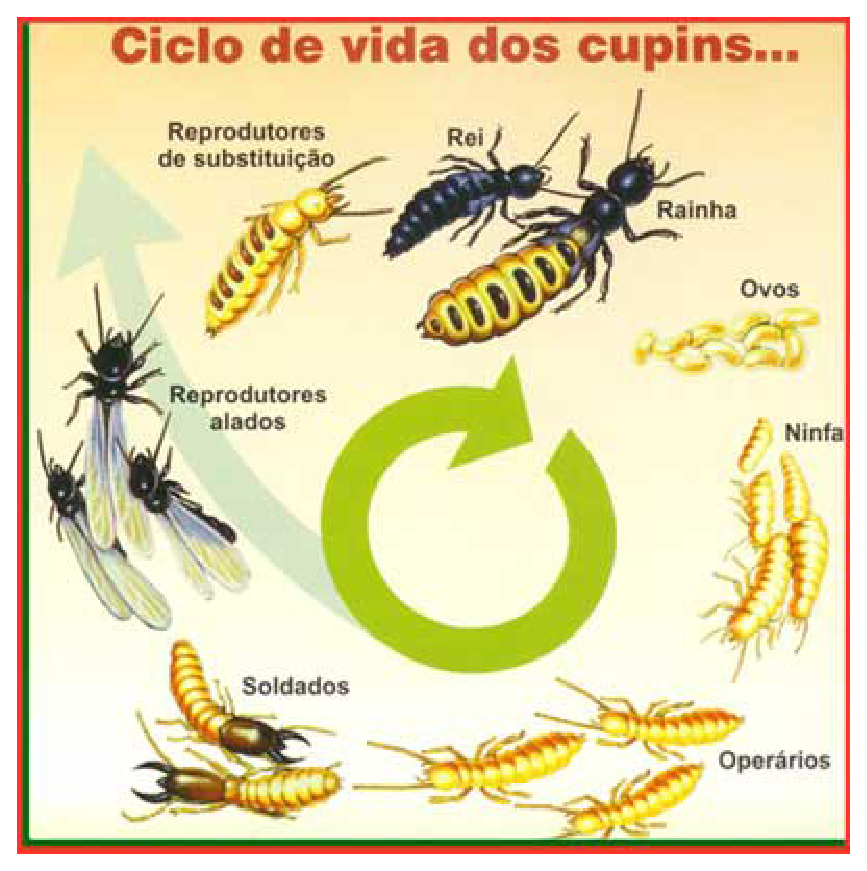
\includegraphics[height=5cm, width=5cm]{texts/ape1/figs/pragas_ciclo_cupim}
    \caption{Uma figura que está no apêndice}\label{FD}
\end{figure}
 % Remover ou comentar
  \chapter{Exemplo de Segundo Ap\^{e}ndice}

\section{Exemplo de Seção do Segundo Ap\^{e}ndice A}

Apêndice e anexos são opcionais no documento. O documento pode conter quantos apêndices ou anexos forem necessários. Lembrando que Apêndice é um documento ou texto elaborado pelo autor a fim de complementar sua argumentação e Anexo é um documento ou texto não elaborado pelo autor que servem de fundamentação ou comprovação (por exemplo: relatórios, mapas, leis, estatutos dentre outros). Os apêndices devem aparecer após as referências, e os anexos, após os apêndices, e ambos devem constar no sumário.
Caso tenha mais do que um apêndice e ou um anexo, deve-se utilizar a nomenclatura: Apêndice A, Apêndice B, Apêndice C etc.

\subsection{Exemplo de Subseção do Segundo Ap\^{e}ndice A}

A matriz de Álgebra Linear $M$ e o vetor de torques inerciais $b$, utilizados na simulação são calculados segundo a formulação abaixo:
\begin{equation}
    M=\left[
        \begin{array}{ccc}
            M_{11} & M_{12} & M_{13} \\
            M_{21} & M_{22} & M_{23} \\
            M_{31} & M_{32} & M_{33}
        \end{array} \right]
\end{equation}

  \annex % Anexos (opcional)
  % Caso anexos não sejam utilizados comentar ou remover os comandos `input`
  \chapter{Exemplo de um Primeiro Anexo}

% Texto do Primeiro Anexo

\section{Uma Seção do Primeiro Anexo}
% Texto da primeira secao do primeiro anexo
Algum texto na primeira seção do primeiro anexo.


  \chapter{Exemplo de um Segundo Anexo}

% Texto do Segundo Anexo

\section{Uma Seção do Segundo Anexo}
% Texto da primeira secao do Segundo anexo
Algum texto na primeira seção do segundo anexo.



  %========================
  =====================================================
  % Definição da Folha de Registro do Documento (FRD)
  %=============================================================================

  % Valores dos campos da FRD

  % Data do registro do documento
  \FRDitadata{26 de março de 2024}

  % Número de registro, fornecido pela biblioteca sob solicitação
  \FRDitadocnro{DCTA/ITA/TD-314/2024}
  \FRDitapalavrasautor{PalavraChave1; PalavraChave2; PalavraChave3}
  \FRDitapalavrasresult{PalavraChave1; PalavraChave2; PalavraChave3}
  % Difícil de usar variáveis pois essa pagina precisa ser sempre em português
  \FRDitapalavraapresentacao{
    ITA, \sjc.
    Curso de \itaoptioncourse.
    Programa de Pós-Graduação em \itaworkcourse.
    Área de \itaworkarea.
    Orientador(a): \itaadvisortitle\ \itaadvisorname.
    Coorientador(a):\ \itacoadvisorname.
    Defesa em 26/03/2024.
    Publicada em 26/03/2024.
  }
  \FRDitapalavraapresentacao{
    ITA, \sjc.
    Curso de XXX.
    Programa de Pós-Graduação em XXX.
    Área de XXX.
    Orientador: \itaadvisortitle\ \itaadvisorname.
    Coorientadora: \itacoadvisortitle\ \itacoadvisorname.
    Defesa em dd/mm/aaaa.
    Publicada em dd/mm/aaaa.
  }
  \FRDitaresumo{Aqui começa o resumo do referido trabalho. O resumo é a versão em Português do {\em abstract}, e como tal, segue as mesmas diretrizes de conteúdo.
}
  %  Primeiro Parâmetro: Nacional ou Internacional -- N/I
  %  Segundo parâmetro: Ostensivo, Reservado, Secreto ou Ultrassecreto -- O/R/S/U
  \FRDitaOpcoes{N}{O}
  % Cria o formulário
  \itaFRD
\end{document}
% Fim do Documento.
